\documentclass[11pt,twocolumn]{article}
\usepackage{graphicx}
\usepackage{hyperref}
\usepackage{fancyhdr}
\pagestyle{fancy}
\fancyhead{}
\fancyfoot{}
\fancyfoot[C]{-\thepage-}
\fancyfoot[L]{Crockford et al}
\fancyfoot[RO]{Scientific Reports:Original Study}
\renewcommand{\footrulewidth}{0.4 pt}
\renewcommand{\headrulewidth}{0 pt}

\hypersetup{colorlinks = true, linkcolor = blue, citecolor = blue}
\title{Investigation into the relationship between B. henselae infection and Feline Uveitis in domestic cats in the United States.}
\author{Student ID: 997900158}
\date{\today}
\begin{document}
\twocolumn[
	\begin{@twocolumnfalse}
	\maketitle
	\begin{abstract}
		This study's objective was to determine if there is an association between \emph{Bartonella sp.} as measured by Western Blot and Feline Uveitis. 
		Medical records were queried from 2 Veterinary Medical Record Databases to find 821 cases of uveitis and 1658 controls.
		The physical examination findings, histories, and diagnostic test results were collected and \emph{Bartonella sp.} exposure status assessed using stored blood samples.


		Cases were 2.1 times more likely to be seropositive for \emph{Bartonella sp.} (p \textless 0.05), and housing status and geographical location were found to modify this effect, probably due to association with flea exposure.


		The results of this study indicate there is a significant relationship between uveitis and \emph{Bartonella sp.} exposure, and support diagnostic testing for \emph{Bartonella sp.} when working up a uveitis case.
	\end{abstract}
\end{@twocolumnfalse}
]

	\section{Introduction}
		Uveitis is inflammation of iris, ciliary body, and choroid of the eye, and is a significant cause of ocular disease in dogs and cats \cite{Townsend2008}. 
		Clinical signs of Uveitis are the same regardless of cause and can include aqueous flare, iritis, keratic precipitates, hyphema, and hypopyon \cite{Powell2010}.


		The causes of uveitis can be grouped into endogenous and exogenous, depending on the nature of disease. Exogenous uveitis is commonly caused by trauma and is easily diagnosed with fluorescein staining of the cornea to indicate ulceration \cite{Fontenelle2008}.
		The most common causes of endogenous feline uveitis include \emph{Bartonella sp.} , toxoplasmosis, feline immunodeficiency virus (FIV), lymphosarcoma (LSA) with or without feline leukemia virus (FeLV), feline infectious peritonitis (FIP), cryptococcosis, neoplasia, and idiopathic causes \cite{Powell2001}.
		Identifying if an infectious agent is responsible for uveitis can be difficult due to the non specific clinical signs, and the lack of adequate diagnostic test \cite{Fontenelle2008}.


		\emph{Bartonella sp.} is a common transient infection in cats, with many not showing any clinical signs. 
		The bacteria is carried by fleas, and kittens commonly become infected while young and go on to develop lifelong immunity.
		On average 20 percent of cats are seropositive to \emph{Bartonella sp.}, although this varies widely with geographic location\cite{Jameson1995a}. Areas that are have a good year-round climate for fleas (warm, humid with mild winters) tend to have higher seroprevalence, indicating the important role played by the fleas in the transmission of this disease.


		\emph{Bartonella sp.} is also an important pathogen from a human health perspective, being responsible for Cat Scratch Disease, which affects 22,000 - 24,000 people annually in the United States, of which approximately 2000 are hospitalised \cite{Jackson1993}.
		\emph{Bartonella sp.} also causes ocular complications in 5 to 10 percent of people that become infected through Cat Scratch Disease \cite{Wade2000}.
	
		Diagnostic tests for \emph{Bartonella sp.} include Serology via Immunofluorescent assay, Enzyme Linked Immunosorbant assay,or Western Blot, and identifying the organism by culture or PCR.
		PCR and culture can be performed on both blood and Aqueous humour, in an attempt to establish causation by locating \emph{Bartonella sp.} at the site of inflammation. Unfortunately \emph{Bartonella sp.} levels in blood and Aqueous humour fluctuate during infection and infected cats may still show a negative test, and hence multiple test are indicated\cite{Guptill2010}. Likewise amplifying DNA from the eye does not necessarily imply causation, and can indicate contamination during sample collection \cite{Powell2010}.


		While cats are generally considered to be subclinical carriers of \emph{Bartonella sp.}, it has been implicated in cases of chronic stomatits, anemia, CNS disorders, and Uveitis \cite{Nasir2005}.
		The association of \emph{Bartonella sp.} and uveitis was first reported by Lappin et al\cite{Lappin1999}, and subsequent studies have found conflicting results, with Ketring reporting increased serum antibodies to \emph{Bartonella sp.} in cats with uveitis\cite{Ketring2004}, while Fontanelle found cats without uveitis more likely to have \emph{Bartonella sp.} antibodies than cats with uveitis.\\
		These studies both had low numbers (251 and 113 cats with uveitis respectively), and did not adequately investigate the effects of geographic location on prevalence of \emph{Bartonella sp.} infection in control cats.
		The proposed biological rationale behind this association can be seen in the attached \hyperref[fig:1]{Causal Diagram}.
	
		This study will utilise large numbers of cats with time, age, housing status, and geographic location recorded, and will determine if a relationship exists between uveitis and seropositivity to  \emph{Bartonella sp.}, in the form of a case control study evaluating records from two large Veterinary Medical record Databases \cite{bark12,UniversityVeterinary}	
		The reference population for this study is privately owned domesticated cats presenting to veterinary hospitals in the United States, and study findings will be generalisable to the ~85 million cats in the United States \cite{HSUSown}.
		

			The Objective of this study is to study the relationship between infection with \emph{Bartonella sp.} and feline uveitis as diagnosed by board certified ophthalmologists.


			The Study Hypothesis is there is a higher incidence of uveitis among cats that have been exposed to \emph{Bartonella sp.}.
\section{Methods}
	Two Veterinary Medical Record databases were queried to locate suitable study participants.
	Banfield is a chain of private veterinary hospitals owned by Mars Inc, and has 770 hospitals located throughout the United States.
	The medical histories of over 2.5 million pets are recorded in a central database \cite{bark12}.
	The Veterinary Medical Database (VMD) features records from 26 university veterinary hospitals located in the United States and Canada, and houses over 6.5 million records \cite{UniversityVeterinary}.
	

	These databases were queried to locate both cases and controls. SQL queries utilising regular expression pattern matching located records of interest by matching keywords, and each record was inspected by the author to determine if it fit study criteria. Because of the large number of records available, any record that was marginally outside parameters detailed below was discarded.
	Records collected between 2012-01-01 and 2012-12-31 were included for analysis in this study.


	Cases of uveitis were diagnosed by a board certified ophthalmologists at either the University Veterinary Hospital or Banfield's In house opthalmology service.
	Case definition was cats presenting with aqueous flare, and at least one of the following clinical signs: blepharospasm, iritis, keratic precipitates, hyphema, and hypopyon. 
	Cases had no mention in their history of evidence of other causes of uveitis including trauma, cataract, intraocular neoplasia, or corneal ulceration (as detected by fluorescein stain) 
	Blood was taken as a part of normal workup of cases and these blood samples are held by the university laboratories for one year following collection. This sample was located, thawed, and submitted to National Veterinary Laboratory to test for \emph{Bartonella sp.} exposure.
	FIV/FeLV exposure status was tested in the normal workup of these cases, and any animal returning a positive result was excluded from this study, as these diseases can also cause uveitis. 
	Any cats undergoing concurrent therapy with glucocorticoids or antibiotics were excluded from the study as glucocorticoid therapy may reduce production of \emph{Bartonella sp.} antibody production \cite{Lappin2000}.
	Age, housing status, geographic location, date of examination, and attending clinician  were also retrieved from the database, 



	Controls were taken from cats visiting Banfield pet hospitals or University General Practices for annual checkups that were found to be healthy. 
	As a part of their checkup, cats are routinely tested for FIV, FeLV, and Toxoplasmosis, and any animal found positive was excluded from this study. 
	Archived blood samples taken for these tests were located, thawed, and submitted to National Veterinary Laboratory to test for \emph{Bartonella sp.} exposure.
	Age, housing status, geographic location, date of examination, and attending clinician  were also retrieved from the database. 
	These cats represent a broad sample of the reference population, that could themselves develop uveitis as a result of \emph{Bartonella sp.} exposure.


	Exposure status was determined with a commercially available Western immunoblot test \cite{febart}. This test is widely used and correlates more closely with the ability to isolate \emph{Bartonella sp.} from cats than does the Immunofluorescent assay or Enzyme Linked Immunosorbant assay \cite{Jr1995}. 
	Western Blot results of 3+ and 4+ were considered positive for the purposes of this study. 
	Results were returned from National Veterinary Laboratory in electronic format and an inner join performed to match exposure status to the study participants.

	The use of an objective exposure method limits the risk of misclassification as both cases and controls will have exposure status determined by the same test.


	Ethical permission was granted by UC Davis School of Veterinary Medicine, and appropriate IACUC forms can be found in the online companion to this article.

	The unit of analysis for this study is the individual cat. 
	Sample size requirements were calculated a control prevalence of 20\%, the average rate as reported by Jameson \cite{Jameson1995a}. Calculations can be seen in \hyperref[fig:samplesizecalc]{Attached code}.
	Sample sizes actually used in this study far exceed those required to establish a biologically significant Odds Ratio difference as calculated above.


	Data integrity was maintained throughout the study using 100\% digital recording and record management. 
	Reproducible workflows were established utilising GNU Make files, documented, and can be found in the online article companion.
	Data quality was strictly enforced, with the use of a large database allowing any incomplete records to be eliminated while maintaining high numbers of study participants.
	Collection of histories by DVM's and Registered Veterinary Technicians ensures quality and consistency, and case diagnosis by qualified ophthalmologists using strict criteria should ensure consistent case definition.


	\subsection{Statistical Evaluation}

		Statistical analysis was initially performed using Fischer's Exact test to compare prevalence rates between cases and control groups. p values of comparison are shown.
		Further modelling was undertaken utilising a conditional logistic regression model, both with and without age, housing status, date of sample collection, and geographical location included. 
		Covariates were included in the final model if the odds ratio for exposure changed by 10\% or more after their addition.
		Geographic location, age, and housing status were included in the final analysis.


		Cats were grouped into 2 age groups (\textless 2, \textgreater 2) as \emph{Bartonella sp.} infection is more common in younger cats
		2 proxies for flea risk were evaluated, housing status (indoor/outdoor) and geographical location.Alaska, Arizona, Colorado, Idaho, Montana, Nevada, New Mexico, Utah, and Wyoming all assigned low risk, all other states high, according to \cite{Jameson1995a}
		Geographical location was assessed at the state level, with each University Veterinary Hospital and surrounding Banfield hospitals forming one category.
		This matching for location ensures comparable case and control populations, removing potential selection bias. 


		Control cats were selected from cats undergoing annual vaccination and checkup, which demonstrates a certain level of care and investment in their animals health by owner. This ensures had their animal shown any signs of uveitis, the owners would probably take their animal to a pet hospital to investigate, and hence come from the same population as cases.


\section{Results}


		Baseline data on study populations can be seen in the attached \hyperref[tab:1]{Table 1} and show the groups are comparable on all baseline characteristics.


		\hyperref[tab:2]{Table 2} shows the results of this study (Odds Ratios and confidence intervals, and p values) with all significant covariates included.
		Initial comparison of seroprevalence rates between cases and controls revealed cats with uveitis had a higher seropositive rate than cats without uveitis ( P-value = 0.02 ) 


		Following the addition of age, housing status, and geographical location, seroprevalence rates were still higher in cats with uveitis, cats housed outdoors, and acts in high risk states (p-values = 0.2, 0.04, 0.01 respectively)
		Age was not found to be significant and hence was not included in the final model.
		Odds ratios (OR) derived from the models were interpreted as measures of increased risk of disease following application of the rare disease assumption ( True uveitis incidence rate is unknown but has been reported at ~ 2\% in the literature.)


\section{Discussion}
		Potential interaction effects of housing status and geographic location were proposed at the beginning of the study and assessed during the analysis stage.
		Odds ratios differed at different geographical locations, as well as with different housing status.
		This seems biologically plausible given the importance of the flea vector in transmission of \emph{Bartonella sp.}, and the documented difference in rates of \emph{Bartonella sp.} seroprevalence across the country \cite{Jameson1995a}.
		Housing status is also a good proxy for flea exposure, with outdoor cats much more likely to be exposed to other cats and environments where they are likely to pick up fleas.
		Both of these interactions were controlled for in the analysis stage of this study and included as a covariate in the final model.

		Potential confounders in this study included age and housing status. 
		Younger cats are more likely to engage in rough play behaviour, and hence develop uveitis due to trauma. Younger cats are also more likely to become infected with \emph{Bartonella sp.}.
		This potential confounder was controlled at the enrolling stage via thorough examination of cases and exclusion if there was any evidence of trauma, either through locating a corneal ulcer through using fluorescein, or any superficial wounds around the facial area.
		Age as a confounder was also controlled at the analysis stage by including it as a covariate in the model.

		
		Housing status is another potential confounder. Cats housed outdoors are more likely to be exposed to fleas and hence have higher seroprevalance rates.
		Outdoor cats are also more likely to experience a traumatic event in the environment, and also more likely to contract FIV/FeLV through interactions with other cats.
		This was controlled in the analysis stage by testing all cases and controls for FIV/FeLV and excluding any positives from the analysis.


		It is possible that misclassification bias resulted in the underreporting of uveitis in the control groups. General practice Veterinarians may not have the training or equipment necessary to identify the signs of uveitis and hence some controls may actually be controls.
		This potential bias was limited by strict inclusion criteria of controls consisting of only cats visiting the hospital for an annual vaccination/checkup. 
		This was further controlled in the analysis stage by querying medical record database and removing any control cats that went on to develop uveitis following the study period.


		Selection bias may have also occurred due to the cats that were included in the study are by definition owned by owners that care about their animals, and are more likely to engage in basic animal husbandry (good diet, regular vaccinations, flea control), and are more likely to notice and attend a veterinarian if any signs of uveitis occur.  
		This source of bias is of little concern however as the reference population for this study is animals reporting to veterinary hospitals so the sample analysed will yield an unbiased estimate of effect.


		Observer bias was also a possibility in the diagnosis of uveitis.
		Rates of uveitis diagnosis was assessed for each board certified ophthalmologist in the study by comparing number of uveitis cases with total number of opthalmologic cases seen per year. This uveitis diagnosis rate was compared to the pooled uveitis diagnosis rate from all ophthalmologists for each facility, and for all ophthalmologist in this study.
		ANOVA analysis revealed a non significant facility and individual effect, suggesting diagnosis was fairly consistent across ophthalmologists.
		In addition, the retrospective nature of this study meant that at the time of diagnosis the practitioner could not have been influenced by the study hypothesis and making was hence not necessary. 


		Temporal Bias was also possibly present in this study due to the nature of \emph{Bartonella sp.} infection and the testing method chosen. 
		Seroprevealce only indicates past exposure to \emph{Bartonella sp.} and does not imply causation in cases of uveitis.
		It is possible that many idiopathic cases of uveitis were falsely attributed to \emph{Bartonella sp.} when the actual \emph{Bartonella sp.} exposure was years before the case of uveitis.


	\subsection{Strengths and Limitations}
		Using cats that were owned by people with  some level of care for their animals is important to make findings generalisable.
		Some previous studies have utilised controls from an animal shelter. Cats in a shelter are much more likely to have been outdoors and exposed to fleas, increasing exposure, and may have increased risk of developing uveitis due to trauma and FIV/FeLV exposure from other cats.
		This study utilised cats admitted for annual vaccination as controls and findings are hence applicable to the many privately owned cats in the United States.

		A major strength of this study is the high data quality maintained throughout record collection and analysis, and the large numbers of cats from a diverse geographical area involved in this study.


		Using indoor/outdoor status as proxy for flea exposure is a potential weakness of this study. 
		This design could be improved with actual flea exposure history from owners, although there is potential for misclassification bias resulting from the stigma surrounding flea infection.
		
		
		The difficulty in coming up with a strict case definition for uveitis is another issue with this study. 
		Board Certified Ophthalmologists are certainly the most qualified to assess cases of uveitis, there is still the possibility of diagnostic criteria differing between clinicians. 
		This is in comparison to other diseases of the eye such as glaucoma (also a potential sequale to uveitis) where an objective test (measuring Intra ocular pressure with tonometry) and strict cutoff value can be utilised to form a consistent case definition.
		This potential weakness was tested as explained above and there were no abnormalities found in uveitis diagnosis rates between ophthalmologists.


		The retrospective nature of this study made it difficult to assess causation as discussed above under potential temporal bias. The retrospective record analysis meant many records were missing the required information to be included in the study.

		
		It is clear there is more work required to further investigate the relationship between feline uveitis and \emph{Bartonella sp.} infection.
\newpage

\begin{figure*}[h!]
	\centering
	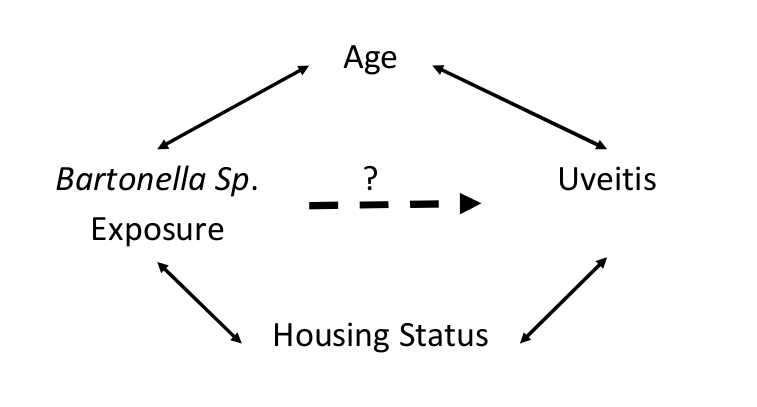
\includegraphics[scale=0.3]{figure1.jpg}
	\caption{Flow Diagram showing proposed Biological Rationale for study, including exposure, outcome and covariates }
	\label{fig:1}
\end{figure*}

\begin{figure*}[h!]
	\centering
	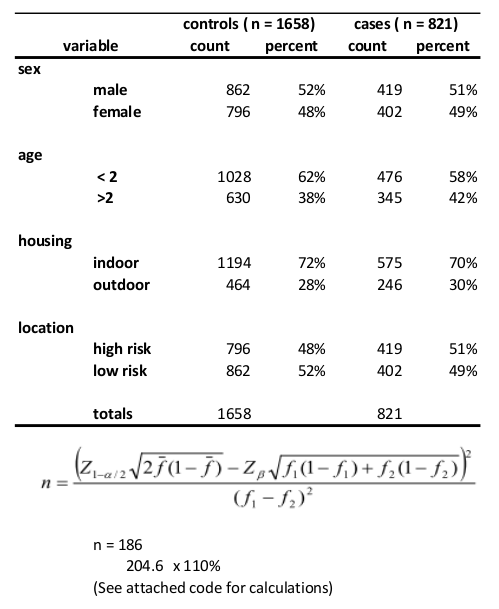
\includegraphics[scale=0.5]{table1.jpg}
	\caption{Characteristics of study participants and sample size calculations.}
	\label{tab:1}
\end{figure*}
 
\begin{figure*}[h!]
	\centering
	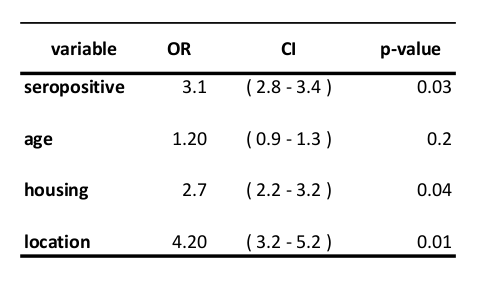
\includegraphics[scale=0.5]{table2.jpg}
	\caption{Odds Ratios (OR) for the association between uveitis and \emph{Bartonella sp.} infection status, age, housing status and geographical location.}
	\label{tab:2}
\end{figure*}

\begin{figure*}[h!]
	\centering
	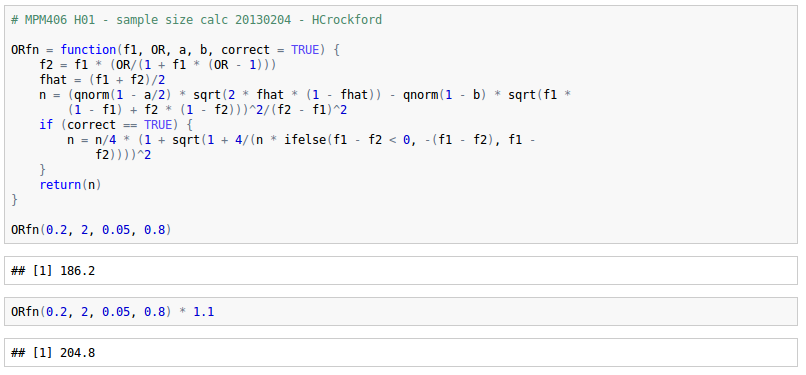
\includegraphics[scale=0.5]{samplesizecalc.jpg}
	\caption{Sample size function and calculation output from R.}
	\label{fig:samplesizecalc}
\end{figure*}

\clearpage
\bibliographystyle{unsrt}
\bibliography{bart.bib}



\end{document}

%%%%%

% interactoins - 
%% make streamlined as possible. but need at least one confounder, not necc any interactions, can say did not find any (kim paper for technique - none stat sig so not included). potential effect modify - wualitative. 
% if include need to show OR with and without interactions.
% table 1 - cats in study,. throw in other factors that wont include - make them the same. e.g. age w exposure outcome and not on causal path. - no sig p value. 
% fig 1 - exposure b \emph{Bartonella sp.} , outcome ev.

% diagram bartonella causing uveitis, age associated w bartonella and uveitis (double ended arrow.) then show in table.( anythign in table that same do not need to have in diagram.
